% Options for packages loaded elsewhere
\PassOptionsToPackage{unicode}{hyperref}
\PassOptionsToPackage{hyphens}{url}
%
\documentclass[
]{article}
\usepackage{lmodern}
\usepackage{amssymb,amsmath}
\usepackage{ifxetex,ifluatex}
\ifnum 0\ifxetex 1\fi\ifluatex 1\fi=0 % if pdftex
  \usepackage[T1]{fontenc}
  \usepackage[utf8]{inputenc}
  \usepackage{textcomp} % provide euro and other symbols
\else % if luatex or xetex
  \usepackage{unicode-math}
  \defaultfontfeatures{Scale=MatchLowercase}
  \defaultfontfeatures[\rmfamily]{Ligatures=TeX,Scale=1}
\fi
% Use upquote if available, for straight quotes in verbatim environments
\IfFileExists{upquote.sty}{\usepackage{upquote}}{}
\IfFileExists{microtype.sty}{% use microtype if available
  \usepackage[]{microtype}
  \UseMicrotypeSet[protrusion]{basicmath} % disable protrusion for tt fonts
}{}
\makeatletter
\@ifundefined{KOMAClassName}{% if non-KOMA class
  \IfFileExists{parskip.sty}{%
    \usepackage{parskip}
  }{% else
    \setlength{\parindent}{0pt}
    \setlength{\parskip}{6pt plus 2pt minus 1pt}}
}{% if KOMA class
  \KOMAoptions{parskip=half}}
\makeatother
\usepackage{xcolor}
\IfFileExists{xurl.sty}{\usepackage{xurl}}{} % add URL line breaks if available
\IfFileExists{bookmark.sty}{\usepackage{bookmark}}{\usepackage{hyperref}}
\hypersetup{
  pdftitle={Results of PangoVis},
  pdfauthor={Devan Becker},
  hidelinks,
  pdfcreator={LaTeX via pandoc}}
\urlstyle{same} % disable monospaced font for URLs
\usepackage[margin=1in]{geometry}
\usepackage{color}
\usepackage{fancyvrb}
\newcommand{\VerbBar}{|}
\newcommand{\VERB}{\Verb[commandchars=\\\{\}]}
\DefineVerbatimEnvironment{Highlighting}{Verbatim}{commandchars=\\\{\}}
% Add ',fontsize=\small' for more characters per line
\usepackage{framed}
\definecolor{shadecolor}{RGB}{248,248,248}
\newenvironment{Shaded}{\begin{snugshade}}{\end{snugshade}}
\newcommand{\AlertTok}[1]{\textcolor[rgb]{0.94,0.16,0.16}{#1}}
\newcommand{\AnnotationTok}[1]{\textcolor[rgb]{0.56,0.35,0.01}{\textbf{\textit{#1}}}}
\newcommand{\AttributeTok}[1]{\textcolor[rgb]{0.77,0.63,0.00}{#1}}
\newcommand{\BaseNTok}[1]{\textcolor[rgb]{0.00,0.00,0.81}{#1}}
\newcommand{\BuiltInTok}[1]{#1}
\newcommand{\CharTok}[1]{\textcolor[rgb]{0.31,0.60,0.02}{#1}}
\newcommand{\CommentTok}[1]{\textcolor[rgb]{0.56,0.35,0.01}{\textit{#1}}}
\newcommand{\CommentVarTok}[1]{\textcolor[rgb]{0.56,0.35,0.01}{\textbf{\textit{#1}}}}
\newcommand{\ConstantTok}[1]{\textcolor[rgb]{0.00,0.00,0.00}{#1}}
\newcommand{\ControlFlowTok}[1]{\textcolor[rgb]{0.13,0.29,0.53}{\textbf{#1}}}
\newcommand{\DataTypeTok}[1]{\textcolor[rgb]{0.13,0.29,0.53}{#1}}
\newcommand{\DecValTok}[1]{\textcolor[rgb]{0.00,0.00,0.81}{#1}}
\newcommand{\DocumentationTok}[1]{\textcolor[rgb]{0.56,0.35,0.01}{\textbf{\textit{#1}}}}
\newcommand{\ErrorTok}[1]{\textcolor[rgb]{0.64,0.00,0.00}{\textbf{#1}}}
\newcommand{\ExtensionTok}[1]{#1}
\newcommand{\FloatTok}[1]{\textcolor[rgb]{0.00,0.00,0.81}{#1}}
\newcommand{\FunctionTok}[1]{\textcolor[rgb]{0.00,0.00,0.00}{#1}}
\newcommand{\ImportTok}[1]{#1}
\newcommand{\InformationTok}[1]{\textcolor[rgb]{0.56,0.35,0.01}{\textbf{\textit{#1}}}}
\newcommand{\KeywordTok}[1]{\textcolor[rgb]{0.13,0.29,0.53}{\textbf{#1}}}
\newcommand{\NormalTok}[1]{#1}
\newcommand{\OperatorTok}[1]{\textcolor[rgb]{0.81,0.36,0.00}{\textbf{#1}}}
\newcommand{\OtherTok}[1]{\textcolor[rgb]{0.56,0.35,0.01}{#1}}
\newcommand{\PreprocessorTok}[1]{\textcolor[rgb]{0.56,0.35,0.01}{\textit{#1}}}
\newcommand{\RegionMarkerTok}[1]{#1}
\newcommand{\SpecialCharTok}[1]{\textcolor[rgb]{0.00,0.00,0.00}{#1}}
\newcommand{\SpecialStringTok}[1]{\textcolor[rgb]{0.31,0.60,0.02}{#1}}
\newcommand{\StringTok}[1]{\textcolor[rgb]{0.31,0.60,0.02}{#1}}
\newcommand{\VariableTok}[1]{\textcolor[rgb]{0.00,0.00,0.00}{#1}}
\newcommand{\VerbatimStringTok}[1]{\textcolor[rgb]{0.31,0.60,0.02}{#1}}
\newcommand{\WarningTok}[1]{\textcolor[rgb]{0.56,0.35,0.01}{\textbf{\textit{#1}}}}
\usepackage{longtable,booktabs}
% Correct order of tables after \paragraph or \subparagraph
\usepackage{etoolbox}
\makeatletter
\patchcmd\longtable{\par}{\if@noskipsec\mbox{}\fi\par}{}{}
\makeatother
% Allow footnotes in longtable head/foot
\IfFileExists{footnotehyper.sty}{\usepackage{footnotehyper}}{\usepackage{footnote}}
\makesavenoteenv{longtable}
\usepackage{graphicx}
\makeatletter
\def\maxwidth{\ifdim\Gin@nat@width>\linewidth\linewidth\else\Gin@nat@width\fi}
\def\maxheight{\ifdim\Gin@nat@height>\textheight\textheight\else\Gin@nat@height\fi}
\makeatother
% Scale images if necessary, so that they will not overflow the page
% margins by default, and it is still possible to overwrite the defaults
% using explicit options in \includegraphics[width, height, ...]{}
\setkeys{Gin}{width=\maxwidth,height=\maxheight,keepaspectratio}
% Set default figure placement to htbp
\makeatletter
\def\fps@figure{htbp}
\makeatother
\setlength{\emergencystretch}{3em} % prevent overfull lines
\providecommand{\tightlist}{%
  \setlength{\itemsep}{0pt}\setlength{\parskip}{0pt}}
\setcounter{secnumdepth}{-\maxdimen} % remove section numbering
\usepackage[]{natbib}
\bibliographystyle{plainnat}

\title{Results of PangoVis}
\author{Devan Becker}
\date{2021-04-11}

\begin{document}
\maketitle

\hypertarget{load-packages-and-data}{%
\section{Load Packages and Data}\label{load-packages-and-data}}

\begin{Shaded}
\begin{Highlighting}[]
\CommentTok{\# Packages that Art hates}
\KeywordTok{library}\NormalTok{(dplyr)}
\end{Highlighting}
\end{Shaded}

\begin{verbatim}
## 
## Attaching package: 'dplyr'
\end{verbatim}

\begin{verbatim}
## The following objects are masked from 'package:stats':
## 
##     filter, lag
\end{verbatim}

\begin{verbatim}
## The following objects are masked from 'package:base':
## 
##     intersect, setdiff, setequal, union
\end{verbatim}

\begin{Shaded}
\begin{Highlighting}[]
\KeywordTok{library}\NormalTok{(tidyr)}
\KeywordTok{library}\NormalTok{(ggplot2)}
\KeywordTok{library}\NormalTok{(stringr)}
\KeywordTok{library}\NormalTok{(here)}
\end{Highlighting}
\end{Shaded}

\begin{verbatim}
## here() starts at /home/devan/OneDriveUWO/0postdoc/sup
\end{verbatim}

\begin{Shaded}
\begin{Highlighting}[]
\NormalTok{dirich \textless{}{-}}\StringTok{ }\NormalTok{params}\OperatorTok{$}\NormalTok{dirich}

\CommentTok{\# Read in CSV files}
\NormalTok{csvs \textless{}{-}}\StringTok{ }\KeywordTok{list.files}\NormalTok{(}\KeywordTok{here}\NormalTok{(}\StringTok{"data/"}\NormalTok{, }\StringTok{"pangolineages"}\NormalTok{),}
    \DataTypeTok{pattern =} \KeywordTok{ifelse}\NormalTok{(dirich, }\StringTok{"*\_d.csv"}\NormalTok{, }\StringTok{"*.csv"}\NormalTok{),}
    \DataTypeTok{full.names =} \OtherTok{TRUE}\NormalTok{)}

\CommentTok{\# Remove any copies}
\NormalTok{csvs \textless{}{-}}\StringTok{ }\NormalTok{csvs[}\OperatorTok{!}\KeywordTok{grepl}\NormalTok{(}\StringTok{"{-}1"}\NormalTok{, csvs)]}

\CommentTok{\# Bring them into one data frame}
\NormalTok{lins \textless{}{-}}\StringTok{ }\KeywordTok{bind\_rows}\NormalTok{(}\KeywordTok{lapply}\NormalTok{(csvs, read.csv))}

\CommentTok{\# Taxon is encoded as \_ACCSESSIONNUMBER.ID, split into ACCESSIONNUMBER and ID}
\NormalTok{lins \textless{}{-}}\StringTok{ }\NormalTok{lins }\OperatorTok{\%\textgreater{}\%}
\StringTok{    }\KeywordTok{separate}\NormalTok{(}\DataTypeTok{col =} \StringTok{"taxon"}\NormalTok{, }\DataTypeTok{sep =} \StringTok{"}\CharTok{\textbackslash{}\textbackslash{}}\StringTok{."}\NormalTok{,}
        \DataTypeTok{into =} \KeywordTok{c}\NormalTok{(}\StringTok{"taxon"}\NormalTok{, }\StringTok{"sample"}\NormalTok{)) }\OperatorTok{\%\textgreater{}\%}
\StringTok{    }\KeywordTok{mutate}\NormalTok{(}\DataTypeTok{taxon =} \KeywordTok{str\_replace}\NormalTok{(taxon, }\StringTok{"}\CharTok{\textbackslash{}\textbackslash{}}\StringTok{\_"}\NormalTok{, }\StringTok{""}\NormalTok{))}

\NormalTok{badlins \textless{}{-}}\StringTok{ }\KeywordTok{table}\NormalTok{(lins}\OperatorTok{$}\NormalTok{taxon)}
\NormalTok{badlins \textless{}{-}}\StringTok{ }\KeywordTok{names}\NormalTok{(badlins[}\KeywordTok{which}\NormalTok{(badlins }\OperatorTok{\textless{}}\StringTok{ }\DecValTok{5000}\NormalTok{)])}
\KeywordTok{cat}\NormalTok{(}\KeywordTok{length}\NormalTok{(badlins), }\StringTok{" runs were removed for having too few samples."}\NormalTok{)}
\end{Highlighting}
\end{Shaded}

\begin{verbatim}
## 11  runs were removed for having too few samples.
\end{verbatim}

\begin{Shaded}
\begin{Highlighting}[]
\NormalTok{lins \textless{}{-}}\StringTok{ }\KeywordTok{filter}\NormalTok{(lins, }\OperatorTok{!}\NormalTok{taxon }\OperatorTok{\%in\%}\StringTok{ }\NormalTok{badlins)}

\CommentTok{\#\#\#\# Visualize the uncertainty in the base calls {-}{-}{-}{-}}
\NormalTok{taxons \textless{}{-}}\StringTok{ }\KeywordTok{sort}\NormalTok{(}\KeywordTok{unique}\NormalTok{(lins}\OperatorTok{$}\NormalTok{taxon))}
\KeywordTok{length}\NormalTok{(taxons)}
\end{Highlighting}
\end{Shaded}

\begin{verbatim}
## [1] 80
\end{verbatim}

\hypertarget{abstract-info}{%
\section{Abstract Info}\label{abstract-info}}

\begin{Shaded}
\begin{Highlighting}[]
\NormalTok{summs \textless{}{-}}\StringTok{ }\NormalTok{lins }\OperatorTok{\%\textgreater{}\%}
\StringTok{    }\KeywordTok{group\_by}\NormalTok{(taxon) }\OperatorTok{\%\textgreater{}\%}
\StringTok{    }\KeywordTok{summarise}\NormalTok{(}
        \DataTypeTok{maxperc =} \KeywordTok{mean}\NormalTok{(lineage }\OperatorTok{==}\StringTok{ }\KeywordTok{names}\NormalTok{(}\KeywordTok{sort}\NormalTok{(}\KeywordTok{table}\NormalTok{(lineage),}
            \DataTypeTok{decreasing =} \OtherTok{TRUE}\NormalTok{)[}\DecValTok{1}\NormalTok{])),}
        \DataTypeTok{uniques =} \KeywordTok{length}\NormalTok{(}\KeywordTok{unique}\NormalTok{(lineage)),}
        \DataTypeTok{minpango =} \KeywordTok{min}\NormalTok{(probability),}
        \DataTypeTok{maxpango =} \KeywordTok{max}\NormalTok{(probability),}
        \DataTypeTok{menpango =} \KeywordTok{mean}\NormalTok{(probability),}
        \DataTypeTok{max =} \KeywordTok{names}\NormalTok{(}\KeywordTok{sort}\NormalTok{(}\KeywordTok{table}\NormalTok{(lineage), }\DataTypeTok{decreasing =} \OtherTok{TRUE}\NormalTok{))[}\DecValTok{1}\NormalTok{])}
\end{Highlighting}
\end{Shaded}

\begin{verbatim}
## `summarise()` ungrouping output (override with `.groups` argument)
\end{verbatim}

\begin{Shaded}
\begin{Highlighting}[]
\KeywordTok{print}\NormalTok{(}\StringTok{"summary info"}\NormalTok{)}
\end{Highlighting}
\end{Shaded}

\begin{verbatim}
## [1] "summary info"
\end{verbatim}

\begin{Shaded}
\begin{Highlighting}[]
\KeywordTok{print}\NormalTok{(summs)}
\end{Highlighting}
\end{Shaded}

\begin{verbatim}
## # A tibble: 80 x 7
##    taxon      maxperc uniques minpango maxpango menpango max      
##    <chr>        <dbl>   <int>    <dbl>    <dbl>    <dbl> <chr>    
##  1 ERR4363387   0.950      19        1        1        1 B.1.222  
##  2 ERR4364007   0.821      84        1        1        1 B.1.1.29 
##  3 ERR4664555   0.963      27        1        1        1 B.1.1.253
##  4 ERR4667618   0.993       7        1        1        1 B.1.1.315
##  5 ERR4692364   0.914      55        1        1        1 B.1      
##  6 ERR4693034   0.869      77        1        1        1 B.1.1.310
##  7 ERR4693061   0.954      19        1        1        1 B.23     
##  8 ERR4693079   0.874      99        1        1        1 B.1.1.310
##  9 ERR4693537   0.973       9        1        1        1 B.1.177.7
## 10 ERR4693605   0.968      15        1        1        1 B.1.177.3
## # ... with 70 more rows
\end{verbatim}

\begin{Shaded}
\begin{Highlighting}[]
\DecValTok{1} \OperatorTok{{-}}\StringTok{ }\KeywordTok{mean}\NormalTok{(summs}\OperatorTok{$}\NormalTok{maxperc); }\DecValTok{1} \OperatorTok{{-}}\StringTok{ }\KeywordTok{mean}\NormalTok{(summs}\OperatorTok{$}\NormalTok{menpango)}
\end{Highlighting}
\end{Shaded}

\begin{verbatim}
## [1] 0.09735665
\end{verbatim}

\begin{verbatim}
## [1] 0.0249975
\end{verbatim}

\begin{Shaded}
\begin{Highlighting}[]
\CommentTok{\#print(summs, n = Inf)}
\end{Highlighting}
\end{Shaded}

\hypertarget{stacked-bar-plots}{%
\section{Stacked Bar Plots}\label{stacked-bar-plots}}

\begin{Shaded}
\begin{Highlighting}[]
\NormalTok{max\_label \textless{}{-}}\StringTok{ }\DecValTok{250}
\NormalTok{other\_label \textless{}{-}}\StringTok{ }\DecValTok{100}

\KeywordTok{par}\NormalTok{(}\DataTypeTok{mfrow =} \KeywordTok{c}\NormalTok{(}\DecValTok{17}\NormalTok{, }\DecValTok{1}\NormalTok{), }\DataTypeTok{mar =} \KeywordTok{c}\NormalTok{(}\FloatTok{0.05}\NormalTok{, }\FloatTok{7.75}\NormalTok{, }\FloatTok{0.05}\NormalTok{, }\FloatTok{0.05}\NormalTok{))}
\ControlFlowTok{if}\NormalTok{ (}\KeywordTok{exists}\NormalTok{(}\StringTok{"seq\_info"}\NormalTok{)) }\KeywordTok{rm}\NormalTok{(seq\_info)}
\ControlFlowTok{for}\NormalTok{ (i }\ControlFlowTok{in} \KeywordTok{seq\_along}\NormalTok{(taxons)) \{}
\NormalTok{    pang \textless{}{-}}\StringTok{ }\NormalTok{lins[lins}\OperatorTok{$}\NormalTok{taxon }\OperatorTok{==}\StringTok{ }\NormalTok{taxons[i], ]}
\NormalTok{    called \textless{}{-}}\StringTok{ }\NormalTok{pang}\OperatorTok{$}\NormalTok{lineage[pang}\OperatorTok{$}\NormalTok{sample }\OperatorTok{==}\StringTok{ }\DecValTok{0}\NormalTok{][}\DecValTok{1}\NormalTok{]}
\NormalTok{    pangtab \textless{}{-}}\StringTok{ }\KeywordTok{sort}\NormalTok{(}\KeywordTok{table}\NormalTok{(pang}\OperatorTok{$}\NormalTok{lineage), }\DataTypeTok{decreasing =} \OtherTok{TRUE}\NormalTok{)}

\NormalTok{    seq\_info\_i \textless{}{-}}\StringTok{ }\KeywordTok{data.frame}\NormalTok{(}
        \DataTypeTok{called =}\NormalTok{ called,}
        \DataTypeTok{mode =} \KeywordTok{names}\NormalTok{(pangtab)[}\DecValTok{1}\NormalTok{],}
            \DataTypeTok{mode\_count =}\NormalTok{ pangtab[}\DecValTok{1}\NormalTok{],}
        \DataTypeTok{runner\_up =} \KeywordTok{names}\NormalTok{(pangtab)[}\DecValTok{2}\NormalTok{],}
            \DataTypeTok{runner\_up\_count =}\NormalTok{ pangtab[}\DecValTok{2}\NormalTok{],}
        \DataTypeTok{unique =} \KeywordTok{length}\NormalTok{(pangtab), }\DataTypeTok{atoms =} \KeywordTok{sum}\NormalTok{(pangtab }\OperatorTok{==}\StringTok{ }\DecValTok{1}\NormalTok{))}
\NormalTok{    seq\_info\_i}\OperatorTok{$}\NormalTok{taxon \textless{}{-}}\StringTok{ }\NormalTok{taxons[i]}

    \ControlFlowTok{if}\NormalTok{ (}\OperatorTok{!}\KeywordTok{exists}\NormalTok{(}\StringTok{"seq\_info"}\NormalTok{)) \{}
\NormalTok{        seq\_info \textless{}{-}}\StringTok{ }\NormalTok{seq\_info\_i}
\NormalTok{    \} }\ControlFlowTok{else}\NormalTok{ \{}
\NormalTok{        seq\_info \textless{}{-}}\StringTok{ }\KeywordTok{bind\_rows}\NormalTok{(seq\_info, seq\_info\_i)}
\NormalTok{    \}}

\NormalTok{    colvec \textless{}{-}}\StringTok{ }\KeywordTok{rep}\NormalTok{(}\StringTok{"grey"}\NormalTok{, }\KeywordTok{length}\NormalTok{(pangtab))}
\NormalTok{    colvec[}\KeywordTok{which}\NormalTok{(}\KeywordTok{names}\NormalTok{(pangtab) }\OperatorTok{==}\StringTok{ }\NormalTok{called)] \textless{}{-}}\StringTok{ "red"}

\NormalTok{    n \textless{}{-}}\StringTok{ }\KeywordTok{sum}\NormalTok{(pangtab }\OperatorTok{\textgreater{}}\StringTok{ }\NormalTok{max\_label)}
    \ControlFlowTok{if}\NormalTok{ (n }\OperatorTok{\textgreater{}}\StringTok{ }\DecValTok{1}\NormalTok{) \{}
\NormalTok{        add\_other \textless{}{-}}\StringTok{ }\OtherTok{FALSE}
        \ControlFlowTok{if}\NormalTok{ (}\KeywordTok{sum}\NormalTok{(pangtab }\OperatorTok{\textless{}}\StringTok{ }\NormalTok{other\_label) }\OperatorTok{\textgreater{}}\StringTok{ }\DecValTok{10}\NormalTok{) \{}
\NormalTok{            add\_other \textless{}{-}}\StringTok{ }\OtherTok{TRUE}
\NormalTok{            other\_count \textless{}{-}}\StringTok{ }\KeywordTok{sum}\NormalTok{(pangtab }\OperatorTok{\textless{}=}\StringTok{ }\NormalTok{other\_label)}
\NormalTok{            pangtab \textless{}{-}}\StringTok{ }\KeywordTok{c}\NormalTok{(pangtab[pangtab }\OperatorTok{\textgreater{}}\StringTok{ }\NormalTok{other\_label],}
                \KeywordTok{c}\NormalTok{(}\StringTok{"other"}\NormalTok{ =}\StringTok{ }\KeywordTok{sum}\NormalTok{(pangtab[pangtab }\OperatorTok{\textless{}=}\StringTok{ }\NormalTok{other\_label])))}
\NormalTok{            colvec[}\KeywordTok{which}\NormalTok{(}\KeywordTok{names}\NormalTok{(pangtab) }\OperatorTok{==}\StringTok{ "other"}\NormalTok{)] \textless{}{-}}\StringTok{ "black"}
\NormalTok{        \}}
\NormalTok{        barlabx \textless{}{-}}\StringTok{ }\KeywordTok{c}\NormalTok{(}\DecValTok{0}\NormalTok{, }\KeywordTok{cumsum}\NormalTok{(pangtab[}\DecValTok{1}\OperatorTok{:}\NormalTok{(n }\OperatorTok{{-}}\StringTok{ }\DecValTok{1}\NormalTok{)])) }\OperatorTok{+}
\StringTok{            }\NormalTok{pangtab[}\DecValTok{1}\OperatorTok{:}\NormalTok{n] }\OperatorTok{/}\StringTok{ }\DecValTok{2}
\NormalTok{        barlabels \textless{}{-}}\StringTok{ }\KeywordTok{names}\NormalTok{(pangtab)[}\DecValTok{1}\OperatorTok{:}\NormalTok{n]}
\NormalTok{        barlens \textless{}{-}}\StringTok{ }\KeywordTok{sapply}\NormalTok{(}\KeywordTok{gregexpr}\NormalTok{(}\StringTok{"}\CharTok{\textbackslash{}\textbackslash{}}\StringTok{."}\NormalTok{, barlabels), length)}
        \ControlFlowTok{for}\NormalTok{ (j }\ControlFlowTok{in} \KeywordTok{seq\_along}\NormalTok{(barlabels)) \{}
            \ControlFlowTok{if}\NormalTok{ (pangtab[j] }\OperatorTok{\textless{}}\StringTok{ }\DecValTok{400} \OperatorTok{\&}\StringTok{ }\NormalTok{barlens[j] }\OperatorTok{\textgreater{}=}\StringTok{ }\DecValTok{2}\NormalTok{) \{}
\NormalTok{                barsplit \textless{}{-}}\StringTok{ }\KeywordTok{strsplit}\NormalTok{(barlabels[j], }\DataTypeTok{split =} \StringTok{"}\CharTok{\textbackslash{}\textbackslash{}}\StringTok{."}\NormalTok{)[[}\DecValTok{1}\NormalTok{]]}
\NormalTok{                barn \textless{}{-}}\StringTok{ }\KeywordTok{length}\NormalTok{(barsplit)}
\NormalTok{                half \textless{}{-}}\StringTok{ }\KeywordTok{floor}\NormalTok{(barn }\OperatorTok{/}\StringTok{ }\DecValTok{2}\NormalTok{)}
\NormalTok{                barlabels[j] \textless{}{-}}\StringTok{ }\KeywordTok{paste0}\NormalTok{(}
                    \KeywordTok{paste}\NormalTok{(barsplit[}\DecValTok{1}\OperatorTok{:}\NormalTok{half], }\DataTypeTok{collapse =} \StringTok{"."}\NormalTok{),}
                    \StringTok{".}\CharTok{\textbackslash{}n}\StringTok{"}\NormalTok{,}
                    \KeywordTok{paste}\NormalTok{(barsplit[(half }\OperatorTok{+}\StringTok{ }\DecValTok{1}\NormalTok{)}\OperatorTok{:}\NormalTok{barn], }\DataTypeTok{collapse =} \StringTok{"."}\NormalTok{)}
\NormalTok{                )}
\NormalTok{            \}}
\NormalTok{        \}}

        \KeywordTok{barplot}\NormalTok{(}\KeywordTok{as.matrix}\NormalTok{(pangtab),}
            \DataTypeTok{col =}\NormalTok{ colvec, }\DataTypeTok{hori =} \OtherTok{TRUE}\NormalTok{, }\DataTypeTok{axes =} \OtherTok{FALSE}\NormalTok{)}
        \KeywordTok{text}\NormalTok{(barlabx, }\FloatTok{0.7}\NormalTok{, barlabels, }\DataTypeTok{cex =} \FloatTok{1.5}\NormalTok{)}
        \ControlFlowTok{if}\NormalTok{ (add\_other) \{}
            \KeywordTok{text}\NormalTok{(}\DataTypeTok{x =} \KeywordTok{sum}\NormalTok{(pangtab) }\OperatorTok{{-}}\StringTok{ }\NormalTok{pangtab[}\StringTok{"other"}\NormalTok{] }\OperatorTok{/}\StringTok{ }\DecValTok{2}\NormalTok{,}
            \DataTypeTok{y =} \FloatTok{0.7}\NormalTok{, }\DataTypeTok{col =} \StringTok{"white"}\NormalTok{, }\DataTypeTok{cex =} \FloatTok{1.5}\NormalTok{,}
            \DataTypeTok{label =} \KeywordTok{paste0}\NormalTok{(}\StringTok{"Others:}\CharTok{\textbackslash{}n}\StringTok{"}\NormalTok{, other\_count))}
\NormalTok{        \}}
        \KeywordTok{mtext}\NormalTok{(}\DataTypeTok{side =} \DecValTok{2}\NormalTok{, }\DataTypeTok{cex =} \DecValTok{1}\NormalTok{, }\DataTypeTok{las =} \DecValTok{1}\NormalTok{,}
            \DataTypeTok{text =} \KeywordTok{paste}\NormalTok{(}\KeywordTok{substr}\NormalTok{(taxons[i], }\DecValTok{1}\NormalTok{, }\DecValTok{3}\NormalTok{),}
                \KeywordTok{substr}\NormalTok{(taxons[i], }\DecValTok{4}\NormalTok{, }\DecValTok{20}\NormalTok{), }\DataTypeTok{sep =} \StringTok{"}\CharTok{\textbackslash{}n}\StringTok{"}\NormalTok{))}
        \KeywordTok{abline}\NormalTok{(}\DataTypeTok{v =} \KeywordTok{seq}\NormalTok{(}\DecValTok{0}\NormalTok{, }\DecValTok{10000}\NormalTok{, }\DecValTok{1000}\NormalTok{), }\DataTypeTok{lty =} \DecValTok{2}\NormalTok{)}
        \StringTok{"pretty\_labels \textless{}{-} seq(0, sum(pangtab),}
\StringTok{                by = ifelse(sum(pangtab) \textless{} 2000, 100, 1000))}
\StringTok{        mtext(side = 1,}
\StringTok{            at = pretty\_labels,}
\StringTok{            text = pretty\_labels,}
\StringTok{            line = 0,}
\StringTok{            cex = 0.75}
\StringTok{        )"}
\NormalTok{    \}}
\NormalTok{\}}

\NormalTok{seq\_info}\OperatorTok{$}\NormalTok{taxon \textless{}{-}}\StringTok{ }\NormalTok{taxons}
\NormalTok{knitr}\OperatorTok{::}\KeywordTok{kable}\NormalTok{(seq\_info, }\DataTypeTok{row.names =} \OtherTok{FALSE}\NormalTok{)}
\end{Highlighting}
\end{Shaded}

\begin{longtable}[]{@{}llrlrrrl@{}}
\toprule
called & mode & mode\_count & runner\_up & runner\_up\_count & unique &
atoms & taxon\tabularnewline
\midrule
\endhead
B.1.222 & B.1.222 & 4756 & B.1 & 108 & 19 & 3 &
ERR4363387\tabularnewline
B.1.1.29 & B.1.1.29 & 4112 & B.1.1.44 & 130 & 84 & 27 &
ERR4364007\tabularnewline
B.1.1.253 & B.1.1.253 & 4819 & B.1 & 52 & 27 & 9 &
ERR4664555\tabularnewline
B.1.1.315 & B.1.1.315 & 4969 & B.1 & 22 & 7 & 2 &
ERR4667618\tabularnewline
B.1 & B.1 & 4577 & B.1.400 & 92 & 55 & 12 & ERR4692364\tabularnewline
B.1.1.310 & B.1.1.310 & 4352 & B.1.1.59 & 185 & 77 & 31 &
ERR4693034\tabularnewline
B.23 & B.23 & 4776 & B.48 & 112 & 19 & 6 & ERR4693061\tabularnewline
B.1.1.310 & B.1.1.310 & 4375 & B.1.1.29 & 212 & 99 & 40 &
ERR4693079\tabularnewline
B.1.177.7 & B.1.177.7 & 4871 & B.1.177 & 125 & 9 & 4 &
ERR4693537\tabularnewline
B.1.177.3 & B.1.177.3 & 4847 & B.1.177 & 62 & 15 & 1 &
ERR4693605\tabularnewline
B.1.36 & B.1.36 & 4724 & B.1.36.9 & 71 & 26 & 8 &
ERR4891711\tabularnewline
B & B & 4408 & B.23 & 189 & 30 & 7 & ERR4891715\tabularnewline
B.1.177.6 & B.1.177.6 & 4944 & B.1.177.9 & 31 & 8 & 1 &
ERR4891805\tabularnewline
B.1 & B.1 & 3736 & B.1.243 & 91 & 216 & 49 & ERR4891841\tabularnewline
B.1.1.216 & B.1.1.216 & 4179 & B.1 & 135 & 132 & 48 &
ERR4891863\tabularnewline
B.1.98 & B.1.98 & 4037 & B.1 & 311 & 75 & 36 & ERR4891889\tabularnewline
B.1.1.304 & B.1.1.304 & 4856 & B.1.1.4 & 16 & 34 & 11 &
ERR4891898\tabularnewline
None & None & 5002 & B.1 & 1 & 2 & 1 & ERR4891916\tabularnewline
B & B & 3401 & B.10 & 609 & 79 & 32 & ERR4891988\tabularnewline
B.1.1.307 & B.1.1.307 & 4975 & B.1 & 10 & 14 & 8 &
ERR4892048\tabularnewline
B.1.1.29 & B.1.1.29 & 1384 & B.1.1.59 & 239 & 213 & 41 &
ERR4892066\tabularnewline
B.39 & B.39 & 4817 & B & 113 & 22 & 8 & ERR4892112\tabularnewline
B.1.177 & B.1.177 & 4372 & B.1.177.7 & 427 & 15 & 3 &
ERR4892152\tabularnewline
B.1.177.17 & B.1.177.17 & 4967 & B.1.177 & 39 & 2 & 0 &
ERR4892200\tabularnewline
B.1.1.216 & B.1.1.216 & 4528 & B.1.1.29 & 38 & 76 & 18 &
ERR4892203\tabularnewline
B.1.1.162 & B.1.1.162 & 3001 & B.1.1.209 & 112 & 198 & 66 &
ERR4892293\tabularnewline
B.1.177 & B.1.177 & 4529 & B.1.177.23 & 181 & 17 & 0 &
ERR4892339\tabularnewline
B.40 & B.40 & 4974 & B & 13 & 7 & 1 & ERR4892386\tabularnewline
B.1.177 & B.1.177 & 4830 & B.1.177.22 & 81 & 17 & 1 &
ERR4892392\tabularnewline
B.1.523 & B.1.523 & 4501 & B.1 & 228 & 30 & 6 &
ERR4892423\tabularnewline
B.1 & B.1 & 4378 & B.1.88 & 140 & 50 & 16 & ERR4893013\tabularnewline
B.1.177 & B.1.177 & 3779 & B.1.177.7 & 985 & 13 & 0 &
ERR4893031\tabularnewline
B.1.1.307 & B.1.1.307 & 4885 & B.1 & 46 & 40 & 22 &
ERR4893033\tabularnewline
B.1.1.29 & B.1.1.29 & 2445 & B.1.1.39 & 101 & 231 & 29 &
ERR4893037\tabularnewline
B.1.177 & B.1.177 & 4819 & B.1.177.22 & 98 & 12 & 4 &
ERR4893080\tabularnewline
B.1.177.16 & B.1.177.16 & 4964 & B.1.177 & 29 & 4 & 1 &
ERR4893138\tabularnewline
B.1.258 & B.1.258 & 4256 & B.1.258.17 & 468 & 24 & 6 &
ERR4893184\tabularnewline
B.1.1.216 & B.1.1.216 & 4441 & B.1.1.208 & 52 & 100 & 43 &
ERR4893186\tabularnewline
B.1.177 & B.1.177 & 4844 & B.1.177.23 & 68 & 17 & 6 &
ERR4893197\tabularnewline
B.1.177 & B.1.177 & 4724 & B.1.177.22 & 131 & 13 & 3 &
ERR4893242\tabularnewline
B.1.1.307 & B.1.1.307 & 4957 & B.1 & 20 & 15 & 10 &
ERR4893353\tabularnewline
B.1.523 & B.1.523 & 4598 & B.1 & 122 & 32 & 7 &
ERR4893393\tabularnewline
B.1.177 & B.1.177 & 4779 & B.1.177.22 & 133 & 21 & 7 &
ERR5062571\tabularnewline
B.1.177.19 & B.1.177.19 & 4914 & B.1.177 & 64 & 8 & 1 &
ERR5063165\tabularnewline
B.1.177 & B.1.177 & 4783 & B.1.177.22 & 115 & 18 & 3 &
ERR5064166\tabularnewline
B.1.1.7 & B.1.1.7 & 5006 & NA & NA & 1 & 0 & ERR5069584\tabularnewline
B.1.1.7 & B.1.1.7 & 5006 & NA & NA & 1 & 0 & ERR5069616\tabularnewline
B.1 & B.1 & 4829 & B.1.247 & 75 & 43 & 14 & ERR5069624\tabularnewline
B.1.1.7 & B.1.1.7 & 5006 & NA & NA & 1 & 0 & ERR5069871\tabularnewline
B.1.177 & B.1.177 & 4841 & B.1.177.22 & 115 & 14 & 2 &
ERR5070060\tabularnewline
B.1.1.7 & B.1.1.7 & 5006 & NA & NA & 1 & 0 & ERR5070294\tabularnewline
B.1.160 & B.1.160 & 4663 & B.1.160.8 & 184 & 17 & 7 &
ERR5074314\tabularnewline
B.1.177.19 & B.1.177.19 & 4875 & B.1.177 & 74 & 13 & 2 &
ERR5076163\tabularnewline
B.1.177.19 & B.1.177.19 & 4852 & B.1.177 & 113 & 12 & 6 &
ERR5076748\tabularnewline
B.1.177 & B.1.177 & 4802 & B.1.177.22 & 114 & 19 & 4 &
ERR5077151\tabularnewline
B.1.1.7 & B.1.1.7 & 5006 & NA & NA & 1 & 0 & ERR5077411\tabularnewline
B.1.1.7 & B.1.1.7 & 5006 & NA & NA & 1 & 0 & ERR5077618\tabularnewline
B.1.36.17 & B.1.36.17 & 4785 & B.1 & 125 & 15 & 5 &
ERR5080897\tabularnewline
B.1.1.311 & B.1.1.311 & 4876 & B.1 & 54 & 14 & 8 &
ERR5080913\tabularnewline
B.1.177 & B.1.177 & 4710 & B.1.177.22 & 130 & 22 & 4 &
ERR5080918\tabularnewline
B.1.177 & B.1.177 & 4667 & B.1.177.22 & 182 & 20 & 5 &
ERR5081301\tabularnewline
B.1.177.4 & B.1.177.4 & 4983 & B.1.177.2 & 11 & 13 & 10 &
ERR5081304\tabularnewline
B.1.177.15 & B.1.177.15 & 4845 & B.1.177 & 130 & 11 & 3 &
ERR5081316\tabularnewline
B.1.177.7 & B.1.177.7 & 3702 & B.1.177 & 1256 & 12 & 1 &
ERR5082556\tabularnewline
B.1.160 & B.1.160 & 4857 & B.1.160.5 & 61 & 15 & 5 &
ERR5082569\tabularnewline
B.1.177 & B.1.177 & 4620 & B.1.177.22 & 240 & 21 & 2 &
ERR5082580\tabularnewline
B.1.177.4 & B.1.177.4 & 4980 & B.1.177.2 & 15 & 8 & 5 &
ERR5082590\tabularnewline
B.1.1.7 & B.1.1.7 & 5006 & NA & NA & 1 & 0 & ERR5082610\tabularnewline
B.1.177.7 & B.1.177.7 & 4879 & B.1.177 & 113 & 10 & 4 &
ERR5082630\tabularnewline
B.1.177 & B.1.177 & 4014 & B.1.177.22 & 391 & 26 & 9 &
ERR5082645\tabularnewline
B.1.1.315 & B.1.1.315 & 4853 & B.1 & 61 & 15 & 6 &
ERR5082664\tabularnewline
B.1.177.6 & B.1.177.6 & 4875 & B.1.177 & 80 & 11 & 2 &
ERR5082674\tabularnewline
B.1.177 & B.1.177 & 4463 & B.1.177.22 & 227 & 19 & 2 &
ERR5082695\tabularnewline
B.1.1.315 & B.1.1.315 & 4403 & B.1.1.281 & 244 & 39 & 18 &
ERR5082696\tabularnewline
B.1.177 & B.1.177 & 3586 & B.1.177.22 & 793 & 30 & 7 &
ERR5082711\tabularnewline
B.1.177.7 & B.1.177.7 & 3240 & B.1.177 & 1704 & 15 & 1 &
ERR5082712\tabularnewline
None & None & 5006 & NA & NA & 1 & 0 & SRR12639958\tabularnewline
A & A & 5708 & B & 2156 & 16 & 0 & SRR12762573\tabularnewline
A.2.2 & A.2.2 & 2950 & A.2 & 730 & 108 & 47 & SRR13020990\tabularnewline
A.1 & A.1 & 8879 & B.40 & 57 & 20 & 6 & SRR13092002\tabularnewline
\bottomrule
\end{longtable}

\begin{Shaded}
\begin{Highlighting}[]
\KeywordTok{rm}\NormalTok{(seq\_info)}
\end{Highlighting}
\end{Shaded}

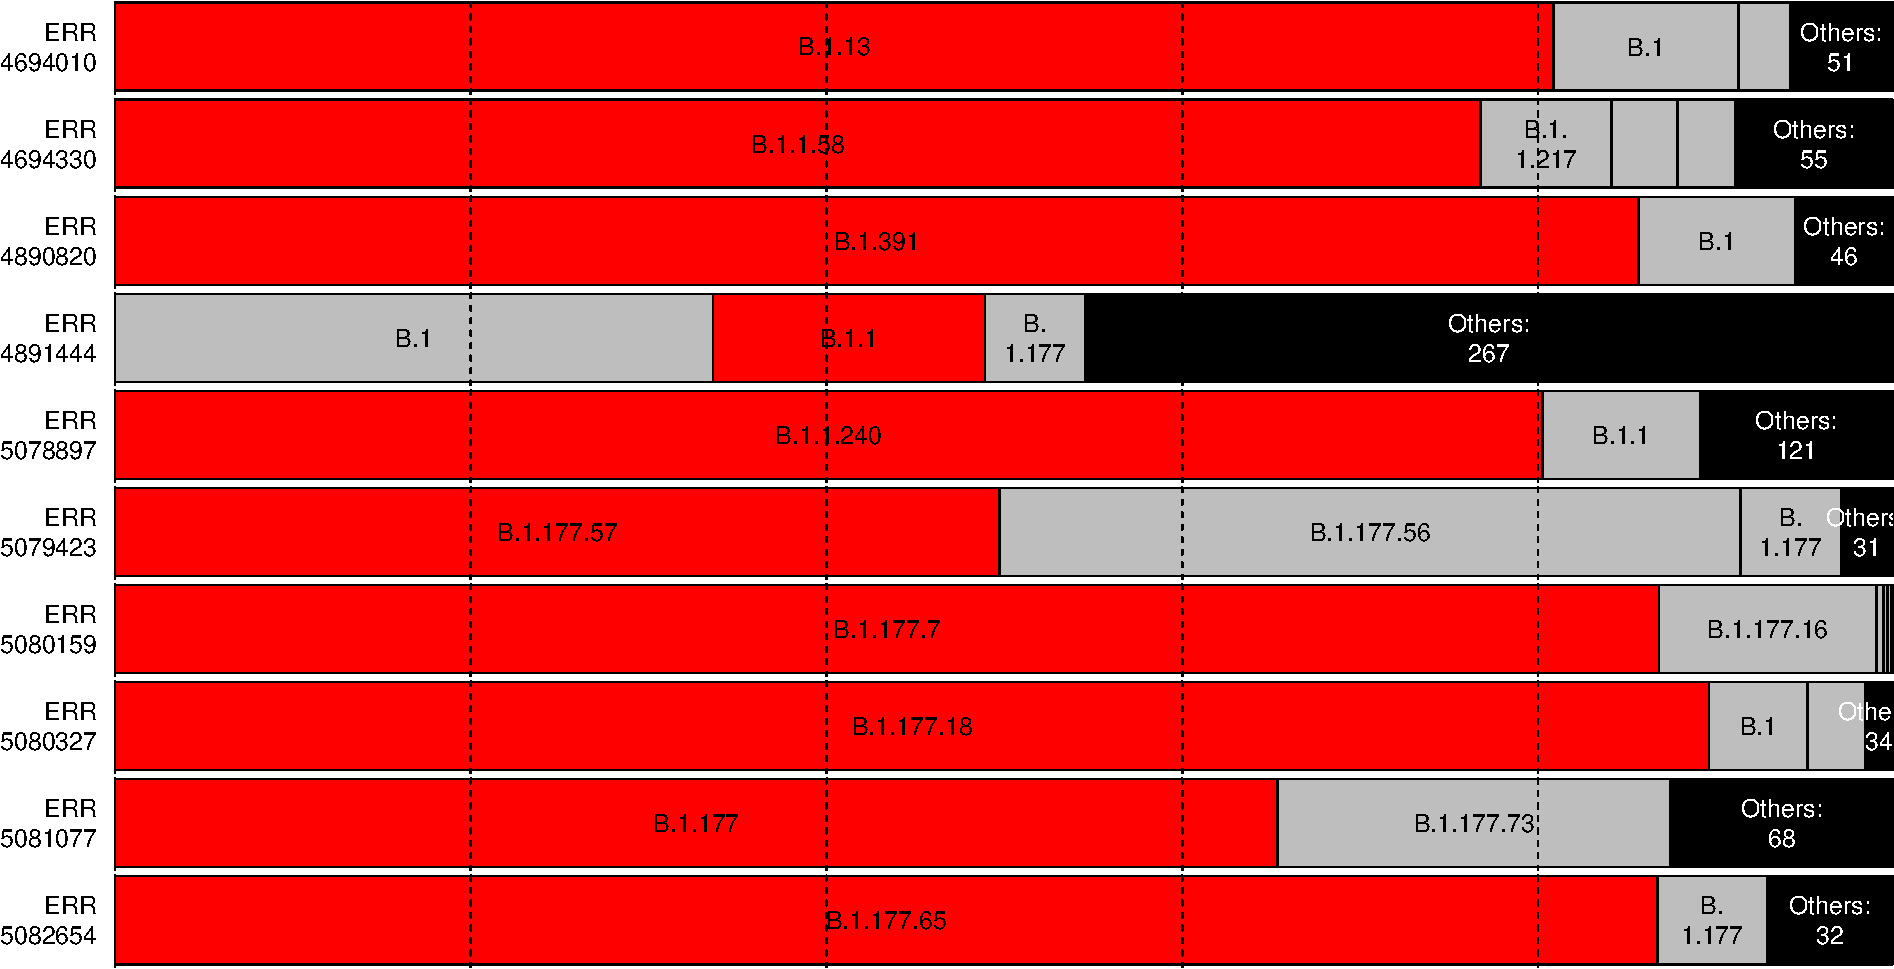
\includegraphics{pangolin_results_report_files/figure-latex/pareto-1.pdf}

\end{document}
